




\subsection{Assurance Monitoring and Control}

\subsubsection{Current Approaches and State-of-the-Art}

Autonomous vehicles need on-line sequential decision making capabilities to successfully complete tasks to meet mission goals. The decision making process needs to produce a sequence of actions that maximizes the expected value of mission utility. The autonomous system uses a system capability model and the environment state estimate to evaluate the potential actions it can take. The system capability model can be represented as a set of parameters; and a search method is required to identify near-optimal action sequences with respect to mission utility.

Consider a scenario where a USV needs to closely follow another vessel. The USV will need to use a hierarchical decision making approach to select the control action~\cite{Shah2016,Bertaska2015,Raboin2015,svec2012automated,svectarget2013,thakur2012}. At the lowest level it will generate a trajectory and use a feedback controller to track the planned trajectory in presence of disturbances. In order to avoid collisions and comply with COLREGS during the execution of planned trajectory, a monitoring  system is necessary. In general, operation time assurance monitoring and control is an essential component of LE-CPS that has to strike the optimal tradeoff between safe execution of actions and achieving mission goals without being extremely conservative.

Unfortunately, complete safety cannot be assured during design time. Similarly, simulation cannot cover all possible cases, and unit and/or end-to-end testing cannot provide guarantees on LECs. Related research also reveals that very few USVs are equipped with on-board monitoring and collision avoidance systems~\cite{naeem2010automatic}. Implementing monitoring systems to meet safety regulations, such as COLREGs imposes further challenges since the rules are often written in plain English for human operators. While a human operator can interpret and employ common sense to abide by these rules, imparting the same capability to an autonomous USV is challenging. 

Capabilities of autonomous system might change due to environmental conditions (e,g., current, waves, wind, etc.). This might affect the trajectory tracking accuracy. The system needs to update its own capability model in a new environment by using safety-aware learning to operate effectively. The on-board perception system might not perform well and might make errors in classification of obstacles. The monitoring system will need to make sure that the classification system is operating over the expected input and should be able to detect cases where the classification system might not work due to lack of training data. 
 
Here, we propose a comprehensive monitoring and control approach that does the following: (a) uses safety-aware learning methods and allows LE-CPS to safely explore new actions/maneuvers without risking the success of missions; (b) monitors architectural and safety constraints; and (c) tracks shifts in distributions. Our monitoring components use the formalism of TA1 and facilitates assurance reasoning by invoking TA3 in a feedback loop.

\subsubsection{Approach}

\begin{figure}[t]
\centering
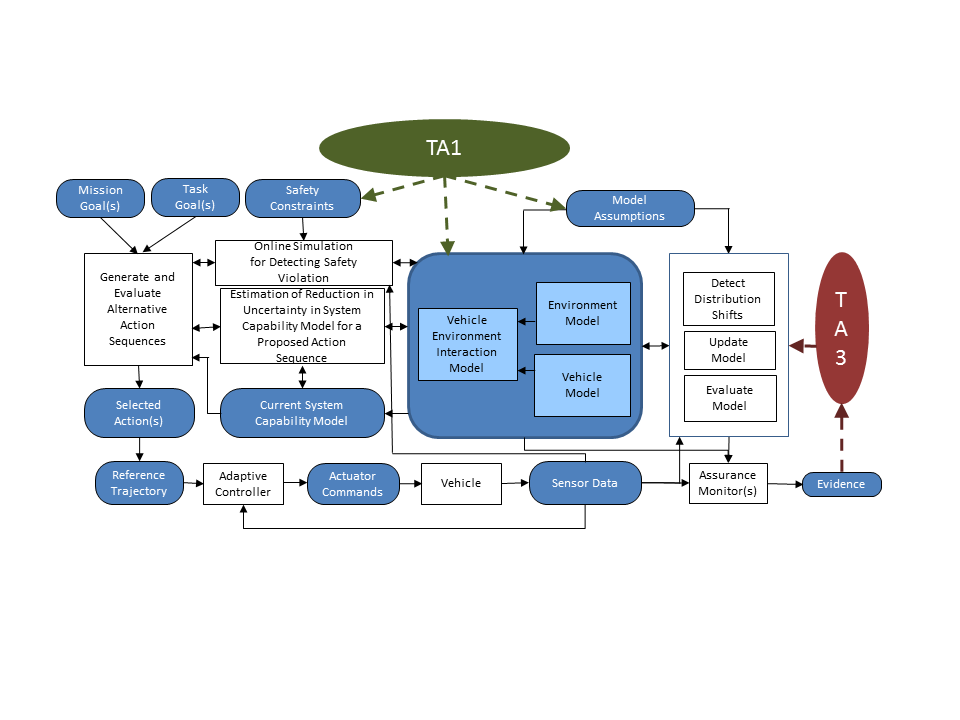
\includegraphics[width=\textwidth,trim=1cm 5cm 0 3cm,clip]{./TA2/sal-v5.png}
\caption{Shows the interactions between various components of TA2.}
\end{figure}

\paragraph{Scalable Safety-Aware Learning}

In most real-world scenarios, there are uncertainties in parameter estimates that describe the system capability model and the obstacles  in the environment. Pre-operation testing can be used to reduce uncertainties for a small number of environment  conditions. However, when the autonomous vehicle encounters a new operational environment for which test data does not exist, uncertainties in parameter estimates increase significantly. For example, consider an autonomous USV that operates in an environment with significant currents, winds, waves, and fog. Any previously used parameter estimates for stopping distance, turning radius, and/or trajectory tracking accuracy will now be far from accurate with uncertainties on them increasing significantly. The system now has the following three options:


\begin{itemize}[leftmargin=*,topsep=3pt]
\setlength\itemsep{0em}
\item It can use conservative parameter values---e.g., the largest possible value of stopping distance---for ensuring safety. This conservative strategy---in the same example---is successful in moving the vehicle very slowly in order to avoid collisions with dynamic obstacles. As new data becomes available, the system tries to improve the underlying dynamics model. However, the system converges to the dynamics model very slowly and hence its performance is poor with respect to the mission goal.      
\item It can suspend the mission temporarily and execute actions/maneuvers that enable it to learn the system capability model under new environmental conditions. But doing so makes the system temporarily unavailable to perform mission-related tasks.
\item It can initially use conservative parameter values to ensure safety. It can then opportunistically use actions that not only make progress towards the mission goals but also enable the learning components to reduce uncertainty in the parameter estimates. This strategy carefully selects safe actions/maneuvers that not only reduce uncertainty in the system capability model but also make progress towards the mission goals. 
\end{itemize}

Recent work in safe learning area computes states that can lead to unsafe situations based on the uncertainty in the dynamics model and only allow control actions that ensure system safety~\cite{Gillula2012,Gillulay2011,Roy2013}. This enables the system to use learning based controllers. Methods have also been developed to ensure that unsafe regions of the state space are not explored during the learning process~\cite{Polo2011,Martinez2015,Mannucci2017}. Gaussian processes based models are often used to learn system dynamics model~\cite{Akametalu2014,Berkenkamp2015,Berkenkamp2016}. Recent work in this area shows that Gaussian Processes in a Dirichlet Process mixture model can handle large changes in system dynamics ~\cite{McKinnon2017}.  

Most of the previous approaches in this area can be viewed as variants of the first two approaches described above. We are interested in pursuing the third approach that can lead to much faster reduction in uncertainty in state estimation without sacrificing safety. Our work will build upon previous work on learning system dynamics and avoiding unsafe states.       

We propose to develop a new on-line learning-enabled decision making framework that enables the system to compose the right sequence of actions/maneuvers to reduce uncertainty in the system capability model opportunistically without suspending the progress towards the mission goals or compromising safety.  Each candidate action/maneuver is evaluated based on three criteria. First, it is evaluated on the risk of violating a safety constraint by performing worst case analysis. Second, it is evaluated on its relevance to the mission goals. Third, it is evaluated on its expected information gain, i.e., reduction in uncertainty, using a surrogate version of the learning component. These three evaluations are combined to produce a cumulative mission utility value for each action/maneuver that drives our learning-enabled decision making. 

We plan to use learning approaches based on Gaussian Process regression to estimate uncertainty in the system capability model. We will select appropriate approaches for estimating uncertainties in classification system based on the selected learning system. The underlying LECs are designed to accept only data that satisfy the monitor and guard conditions. By design, our framework also discards actions/maneuvers that violate safety constraints. The system will utilize a learning framework that will ensure that the known model structure is utilized to guide the learning process by enforcing the model structure constraints. The learning process will also ensure that the data violating modeling assumption does not corrupt the model, but if appropriate is used to update uncertainty estimates.     

The safety-aware learning module faces the combinatorial problem of generating and evaluating sequences of actions that have to heed to safety constraints, mission goals, and information gain. Because uncertainties associated with the parameters are time-varying and trajectory-dependent, existing approaches are unlikely to be scalable. We therefore propose to develop new scalable search strategies to solve this problem efficiently. The problem of generating and evaluating sequences of actions can be posed in several frameworks, including a branch-and-bound search framework like Anytime A*, or an Markov decision processes (MDP) framework like a finite-horizon MDP. We plan to evaluate FastMap, a recently developed method by our group at USC, that can significantly improve the efficiency of the algorithms in the search framework as well as in the MDP framework~\cite{cujakk}.

While in many application domains, heuristic search begins after the specification of the start and goal states, FastMap preprocesses the extensional or intensional graphs over which search is carried out.  By efficiently embedding nodes in Euclidean space, FastMap preprocesses a graph in near-linear time and produces admissible and consistent heuristics. For example, A* with FastMap heuristics produces optimal solutions 30-40 times faster than many other commonly used heuristics. If the available computational time requires us to use anytime search algorithms to accept suboptimal solution from mission utility point of view, the use of improved heuristics will lead to significantly better quality solutions. Using FastMap the Euclidean embedding can be precomputed in near-linear time for any update to the parameters of the vehicle-environment interaction model.

In finite-horizon MDPs, the same principle can be used to improve the performance of Value Iteration. FastMap can be used to preprocess and transform  the state space of an MDP  into an artificially created Euclidean space in near-linear time. Given a new mission goal, or any set of goal states, the Euclidean distances to their corresponding points is used as an initialization for each state. Value Iteration using FastMap is expected to converge much faster since its initialization and Bellman updates are based on better information.   

\paragraph{Scalable Assurance Monitoring}

An important component of TA2 is the ability to monitor architectural and safety constraints for assurance. Consider the assurance monitoring of an architectural constraint on the coefficient of friction $\mu$. Suppose $\mu$ is modeled to be independent of the velocity $v$ under the assumption that $v$ is always less than a threshold velocity $v_{T}$. While this physical model is fairly accurate, it holds only under the assumption that $v \le v_T$, therefore the constraint has to be continually monitored. Similarly, consider a safety constraint of the USV having to maintain a safe distance of at least $\delta$ from an obstacle. Monitoring architectural and safety constraints accounts for a lot of computational processing since each  constraint has to be checked over and over again as a massive amount of sensor information continually flows in.

To increase the scalability of the monitoring algorithms, we propose novel techniques that we have successfully used in DARPA's RSPACE program. Our systematic use of a physical model of the autonomous vehicle also enables us to monitor architectural and safety constraints much more efficiently. In the same example, suppose we know that the USV has a maximum acceleration of $a_{\max}$. At any time $t$, if the velocity is $v_t < v_T$, we can conclude that it would require at least $\frac{v_T - v_t}{a_{\max}}$ time units to violate the architectural constraint. Therefore, no sensor information needs to be processed until time $t + \frac{v_T - v_t}{a_{\max}}$ for checking this constraint. At time $t + \frac{v_T - v_t}{a_{\max}}$, if the USV indeed has a velocity $v_T$, i.e., if it is on the verge of violating the architectural constraint, an appropriate control action is taken to avert the situation. If not, the USV has a velocity $v < v_T$; and the same reasoning can be applied recursively to compute the next point of time when the sensor information would really matter. This recursive reasoning procedure reduces the amount of sensor information that has to be processed in monitoring  constraints. We have used similar constraint monitoring techniques in DARPA's RSPACE program to extract exponential increases in computational efficiency.

We envision two viable extensions of our current work to the objectives of TA2. First, we can extend it to uncertain environments where variables may or may not be controlled adversarially. Our approach in this context is very principled and is based on the idea of Variable Elimination (VE) in Artificial Intelligence (AI). VE is successfully used is many areas of AI, including constraint satisfaction, probabilistic reasoning, and hierarchical planning. Using VE, an architectural or safety constraint that involves a mix of observable/unobservable, controllable/uncontrollable, and discrete/continuous variables can be reduced to a substrate constraint that characterizes a dominant strategy of the controllable variables over the unobservable and uncontrollable variables. In the case of USVs, for example, the theory of VE provides a principled solution to how architectural and safety constraints can be efficiently monitored in either congenial circumstances, adversarial conditions, or for COLREGs.

The second important extension of our work is in the dynamic assessment of assurance case (DAAC) for TA3. Once again, the idea is to invoke the DAAC only when needed and not at all times when conditional evidence is available. The same kind of reasoning explained above can be used to detect the time intervals during which DAAC is not required. Doing so is expected to improve the scalability by orders of magnitude not only by decreasing number of DAAC initiations but also the communication between the TA2 and TA3 components.


\paragraph{Detecting Distributional Shifts}

When the LE-CPS is running in operational mode, its performance can change significantly if the distribution of the live data differs from that of the training data. These shifts may be caused by physical changes in the environment, adversaries trying to actively defeat the system, or faulty sensors. In general, there are four broad categories of reasons for distributional shifts. First, they can come from sensor failures. Second, they can come from modeling incompleteness such as, inaccurate models for wake dynamics in the USV domain. Third, they can come from a change of conditions between training data and live data, e.g., when the USV starts operating under dense fog, for which no training data was available. Fourth, they can come from physical changes to the vehicle, like deformation in one of the propeller blades, that necessitate  changes to the vehicle-environment interaction model.

Our distribution shift detector continually monitors the distributions, detects any shifts, identifies the category and cause, invokes dynamic assurance,  and either updates the model or raises an alert. We propose to build on our DARPA BRASS effort, where we developed an approach to detect sensor changes and failures and distinguish them from distributional shifts caused by other factors. We do this by learning the relationships among sensors from historical data and then exploiting their relationships to detect failures and deviations. Compared to many existing methods based on change-point/outliers detection~\cite{basseville1993detection,gustafsson2000adaptive,brodsky2013nonparametric,aminikhanghahi2016survey}, our approach is different because it leverages relationships between multiple sensors. Although~\cite{dereszynski2012probabilistic,dietterich2012machine,dereszynski2011spatiotemporal} also leverage such relationships, our approach is capable of examining different combinations of sensors and extracting only a small set of linear or nonlinear relationships between sensors.

In the second case, if no actions have been taken to avert the violation of a modeling assumption or an architectural constraint, we temporarily resort to a safe mode of operation. In the third case, we begin training on data gathered from the new environment and accumulate enough such data to train a new model without any structural changes to it. Here, we rely on the power of modern LECs to quickly enable this transition. In the fourth case, we make structural changes to the model using LECs and their concomitant stochastic contracts provided by TA1.

In operational mode, it is impractical to store all sensor data and use historical information for detecting distributional shifts. We therefore propose to develop a four-fold approach to detect distributional shifts efficiently. One, we test the basic general bounds on the tail probability of an input variable, defined by Markov, Chebyshev, and Chernoff inequalities~\cite{gama2010knowledge}. Two, we extend the algorithms that track statistics and detect changes over a sliding window, such as ADWIN~\cite{bifet2007learning}, by incorporating knowledge from the physical models to reduce computational costs. Three, we adopt commonly-used data reduction techniques, such as sampling, synopses and histograms, wavelets, and discrete Fourier transforms, to detect distributional shifts using compact representations of data~\cite{chan1999efficient,witten2016data}. Four, we explore the potential applicability of modern ML classifiers~\cite{quionero2009dataset} and ensemble-based methods~\cite{Wang:2003:MCD:956750.956778} to identify these distributional shifts.

%\subsection{Detecting Distributional Shifts} 
%When the LE-CPS is running in operational mode its  performance can degrade significantly if the  distribution of the live data differs from the trained data.  There may be a change in the  distribution of input variables between training and test set (covariate shift) or the joint distribution between input and output variables may vary (dataset shift). These shifts may be caused by changes in the  world behavior making the  training distributions  no longer reflective of current reality, adversaries trying to game the systems, or faulty sensors.  Our detection shift module will continuously monitor the distributions, detect any shifts, identify the type and cause, and either update the model or raise an alert. 

%In operational mode the data produced will be unbounded in length making it impractical to store all data and compare with historical information. We plan to develop a four-fold approach to detect distribution shifts. 1) Test the  basic general bounds on the tail probability  of a input variable  defined by Markov, Chebyshev and Chernoff inequalities\cite{gama2010knowledge}.  2) Extend algorithms that track statistics and detect changes over a sliding window, such as ADWIN  \cite{bifet2007learning}, by incorporating knowledge from physical models to reduce the computational costs.  3) Adopt commonly-used data reduction techniques, such as sampling,  synopsis and histograms, wavelet, and discrete Fourier transforms, which provide compact representation to detect shifts \cite{chan1999efficient},\cite{witten2016data}. 4) Employ machine-learning classifiers \cite{quionero2009dataset} and ensemble based methods \cite{Wang:2003:MCD:956750.956778} to identify the shifts in this domain.

%We will build on our DARPA BRASS effort, where we developed an approach to detect sensor changes and failures and distinguish them from distributional shifts that are caused by  environment changes (e.g. seasonal changes for weather sensor data). We do this by learning the relationships among sensors from historical data and then exploit the relationships to detect failures and deviations.  Compared to most existing work in change-point/outliers detection \cite{basseville1993detection,gustafsson2000adaptive,brodsky2013nonparametric,aminikhanghahi2016survey}, our approach is unique in terms of effectively leveraging relationship among multiple sensors. Although \cite{dereszynski2012probabilistic, dietterich2012machine,dereszynski2011spatiotemporal} also leverage sensor relationship, our approach is capable of learning more complicated relationship among sensors, and exploring different types of relationship at the same time. 

%Our algorithm attempts to extract the relationship among sensors by reconstructing one sensor from the other ones. Suppose there are $K$ sensors, and denote the reading of $k$th sensor at time $t$ as $x_k(t)$. Our algorithm may be able to derive the following relationship from data:
%\begin{align} $x_3(t) \approx 3 x_1(t) - 1.5 x_2(t)^2 + 0.8$,
%\end{align} which reconstructs $x_3(t)$ using $x_1(t)$ and $x_2(t)$. The above form can be turned into the following inequality constraint: 
%\begin{align} $\| x_3(t) - 3 x_1(t) + 1.5 x_2(t)^2 - 0.8 \|^2 \leq \epsilon^2$,
%\end{align} where $\epsilon^2$ denotes an error bound that can also be derived from historical data. Our algorithm is capable of examining different combinations of sensors, and extracting a small set of such constraints that capture nonlinear relationship among sensors. Among all possible constraints, our algorithm favors those with fewer number of sensors involved and smaller error bounds.  


%% We propose to build on our work in DARPA BRASS project, where we developed an approach to detect distributional shifts in sensor data  can be caused by  failures and environment changes (e.g. seasonal changes for weather sensor data). To detect distributional shifts, one may first estimate the distribution of current sensor data and then determine whether it's different from the previous one. The challenge is that distribution estimation often requires a significant amount of samples, which does not enable fast detection. Our approach to detect distributional shifts is based on monitoring the relationship among sensors. We learn the sensor relationship from historical data, and use that to capture joint patterns of sensor data. Then we examine each new set of sensor readings. If they violate the learned sensor relationship, then a potential distributional shift is detected.

%% Compared to most existing work in change-point/outliers detection \cite{basseville1993detection,gustafsson2000adaptive,brodsky2013nonparametric,aminikhanghahi2016survey}, our approach is unique in terms of effectively leveraging relationship among multiple sensors. Although \cite{dereszynski2012probabilistic, dietterich2012machine,dereszynski2011spatiotemporal} also leverage sensor relationship, our approach is capable of learning more complicated relationship among sensors, and exploring different types of relationship at the same time.

%% Our detection approach consists of three components:

%% {\bf Learning sensor relationship from historical data:} Given a set of historical sensor data, our algorithm attempts to extract the relationship among sensors by reconstructing one sensor from the other ones. Suppose there are $K$ sensors, and denote the reading of $k$th sensor at time $t$ as $x_k(t)$. Our algorithm may be able to derive the following relationship from data:
%\begin{align}
%%$x_3(t) \approx 3 x_1(t) - 1.5 x_2(t)^2 + 0.8$,
%\end{align}
%which reconstructs $x_3(t)$ using $x_1(t)$ and $x_2(t)$. The above form can be turned into the following inequality constraint: 
%\begin{align}
%$\| x_3(t) - 3 x_1(t) + 1.5 x_2(t)^2 - 0.8 \|^2 \leq \epsilon^2$,
%\end{align}
%where $\epsilon^2$ denotes an error bound that can also be derived from historical data. Our algorithm is capable of examining different combinations of sensors, and extracting a small set of such constraints that capture nonlinear relationship among sensors. Among all possible constraints, our algorithm favors those with fewer number of sensors involved and smaller error bounds.

%% {\bf Detecting changes in sensor relationship.} Given newly observed sensor data, our algorithm checks each constraint to see whether the corresponding error bound is violated or not. If the amount of violation is above a threshold, then our algorithm considers a distributional shift.

%% {\bf Inferring if a sensor has failed.} It is important to determine whether a failed sensor is the cause of a distributional shift. This allows our learning system to understand the root cause of change, as well as provides potential ways to qualify the impact of the change to the learning system (discussed below). To infer the failed sensors, our algorithm explores the following property: if a constraint is violated, then at least one sensor involved in the constraint is likely to have failed. The inference problem can then be solved using reasoning techniques over logical expressions. 

%% When a distributional shift is detected, we are interested in qualifying the impact to the learning system. One idea is to simulate more sensor data based on the observed one and then use such data to test the learning system. The simulation is generally challenging because it may require a large amount of data to model the current distribution, especially when the number of sensors is large. However, if the failed sensors can be accurately identified by our detection algorithm, we only need to model a small set of sensors which may require significantly fewer data points.

%%--


%When a distributional shift is detected, then multiple actions are possible. By learning these relationships, we can determine whether a failed sensor is the cause of a distributional shift. This allows our monitor to understand the root cause of a change, and recover from the change by either constructing a replacement sensor or issuing an alert due to a distribution shift caused by a change in the environment. 
%If a sensor has failed and if combination of other sensors will provide proxy data it will be fed to the model. For temporary shifts \textcolor{red}{TODO: What do we do with temporary and long term drifts, when does it go to assurance monitor, when is learning invoked, What if LEC has multiple models, how do we change them. Discuss with S.K}

\begin{table}[ht]
\caption{Project Plan for TA2}
  \centering
  {\footnotesize
\begin{tabular}{|m{.6in}|m{5.55in}|} 
\hline
\textbf{Phase} & \textbf{Plan} 
\\\hline
Phase I & 
Implement system with 2 LECs and code-level optimizations to reduce the monitoring overhead to 50\%. Explore and implement framework for safety-aware learning. Adapt models and systems defined by TA1. Extend sensor failure detection in BRASS effort to detect distributional shifts. Develop APIs for integration with TA1 and TA3. \\
\hline
Phase II & 
Implement FastMap and heuristic Bellman updates to boost safety-aware Reinforcement Learning. Incorporate physical models of vehicle-environment interactions to allow scaling up to 4 LECs and reduce monitoring overhead to 30\%. Extend sliding window and sampling-based techniques to detect distributional shifts.  \\
\hline
Phase III & 
Focus on proposed novel algorithmic techniques to allow scaling up to 6 LECs and reduce monitoring overhead to 10\%. Add features necessary to support physical trials. \\\cline{1-2}
\hline
\end{tabular}
}
\end{table}


\begin{table}[ht]
\caption{How TA2 Interfaces with TA1 and TA3}
  \centering
  {\footnotesize
\begin{tabular}{|m{.25in}|m{5.90in}|} 
\hline
\textbf{TA2} & \textbf{Interfaces and Interaction} 
\\\hline
TA1 & 
\begin{itemize}[itemsep=0pt,leftmargin=*]
\item\textit{ Delivery interface} to accept fully implemented designs including all executables, libraries, and models along with an interface to review the version of deployed components and monitors.
\item \textit{Monitoring interface} to specify the variables to monitor along with specifications on how to monitor,  such as the monitoring frequency and functions..
\item \textit{Constraints interface} to provide distributions of monitoring variables, constraints, and state machines to implement monitoring capabilities.  
\item \textit{Safety templates} to specify  actions, switch modes, and apply remedial actions schemes while assuring safety of the mission.
\end{itemize} 
\\\hline
TA3 & 
\begin{itemize}[itemsep=0pt,leftmargin=*]
\item TA2 will provide  evidence, conditional evidence, and relevant sensor data.
\item An API to specify when to collect evidence, access historical evidence and sensor data.
\item An API for reporting  Assurance Measures.
\end{itemize}
\\\hline
\end{tabular}
}
\end{table}

\begin{table}[ht]
\caption{Technical Challenges and Mitigation Approach for TA2}
  \centering
  
{\footnotesize
\begin{tabular}{|m{2.7in}|m{3.45in}|} 
\hline
\textbf{Technical Challenge} & \textbf{Mitigation Approach} 
\\\hline
Interpreting the designs and monitors produced by TA1 could be challenging.  &   Develop APIs to specify designs and monitors  early in the program.\\ \hline
Action selection problem is computationally challenging in the presence of multiple learning enabled components and the approach produces sub-optimal decisions for applications requiring fast decision making &  Use multi-resolution adaptive action primitives to speed up the search.  Explore the use of parallel computing to speed up the search process by using multi-core architecture.\\ \hline
Detecting safety constraint violation using on-line simulation is too slow.
 & 
Use conservative approximation to develop simplified simulation that can run fast.
\\ \hline
Models produce large uncertainties and uncertainty reduction process is very slow. & 
Develop specialized sequence of actions to rapidly  reduce uncertainty  and use them as meta-actions during search. \\
\hline
\end{tabular}
}
\end{table}

